\chapter{Om at lave figurer} \label{kap:figurer}

Man kan nemt indlejre grafikfiler med \texttt{graphicx}-pakken, der
tilbyder bla. \verb2\includegraphics2-kommandoen.

Se \fig{fig:lamport} og læg mærke til, hvordan vi skalerer
billedfilen, så den ere 7 centimeter bred i teksten.

\begin{figure}[h]
  \centering
  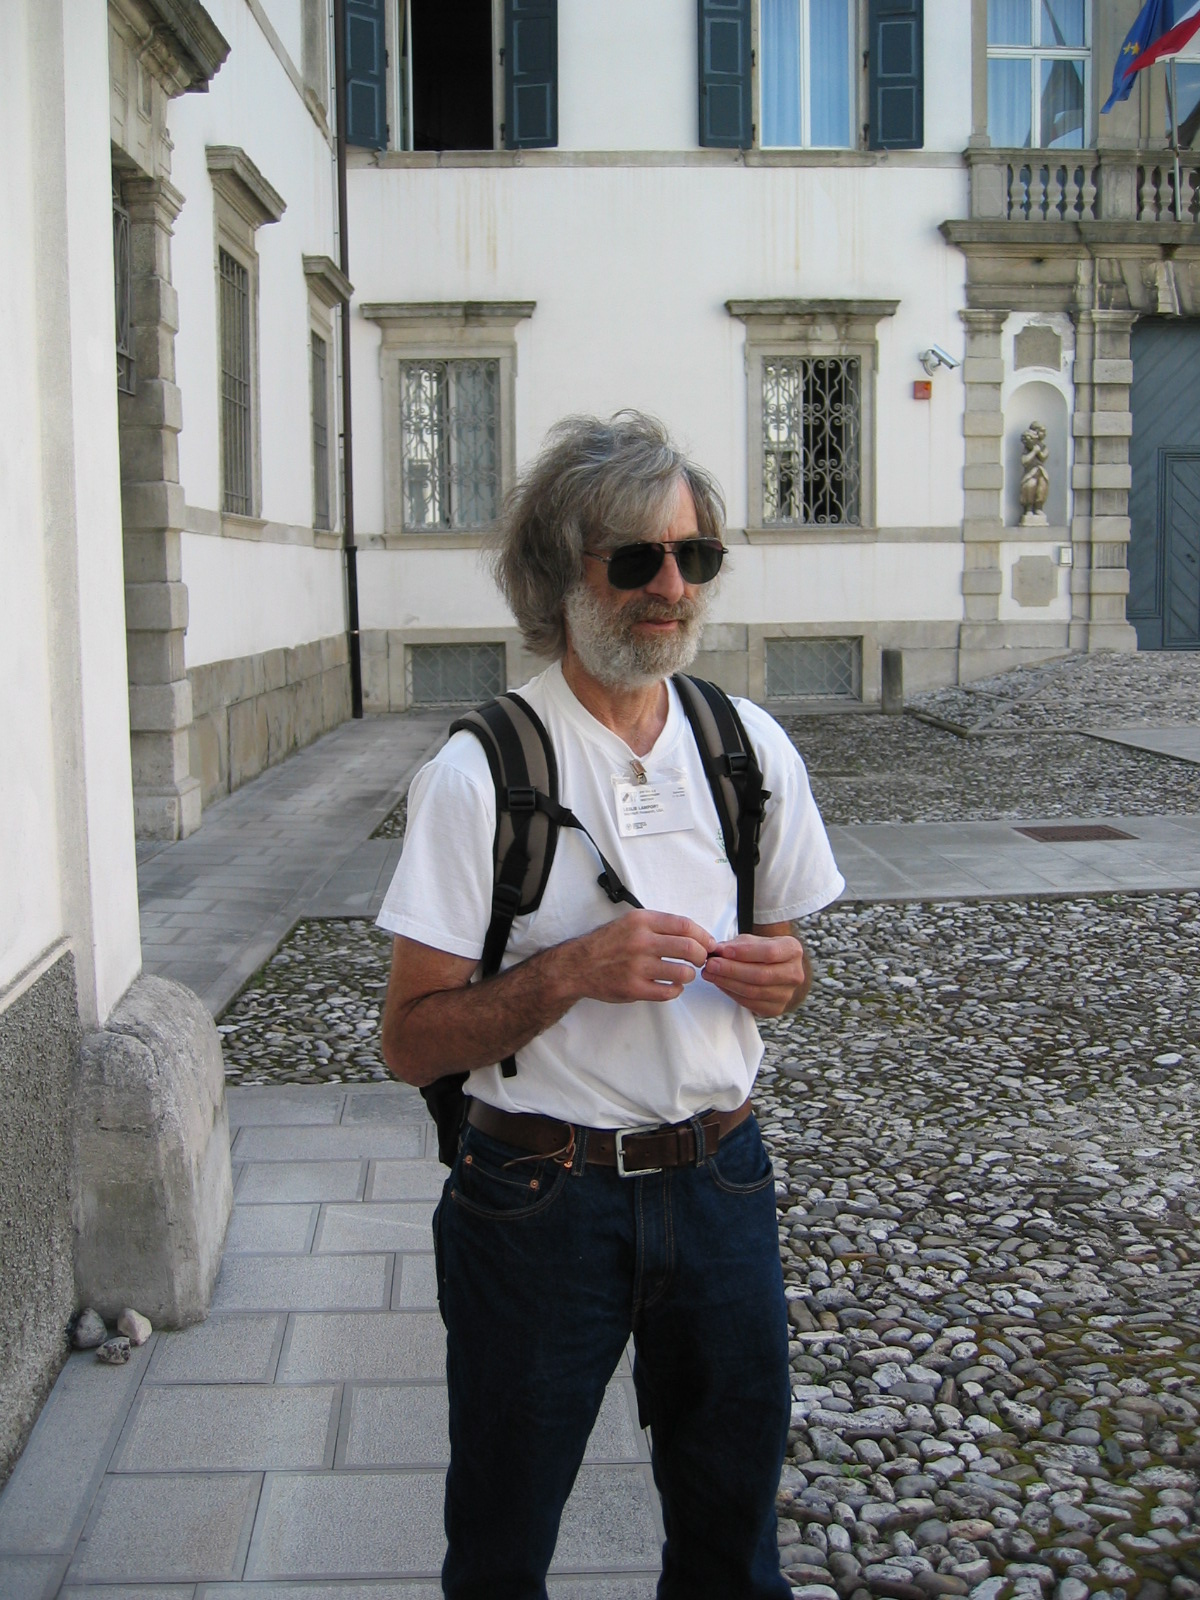
\includegraphics[width=7cm]{figurer/lamport}
  \caption{Leslie Lamport}
  \label{fig:lamport}
\end{figure}

\texttt{tikz} er en pakke, der gør det muligt at beskrive vektorgrafik -- det
er et helt lille programmeringssprog. Figur \ref{fig:tm}
viser et eksempel, der ligger i en særskilt fil (indlæst med
\verb2\input2-kommandoen). 

\begin{figure}[h]
\begin{tikzpicture}[>=latex',join=bevel,]
\tikzstyle{every state}=     [draw=black!50,very thick,fill=gray!20]%
 \node (q0) at (50bp,320bp) [state, initial]{$q_0$};
 \node (q1) at (200bp,320bp) [state]{$q_1$};
 \node (q2) at (350bp,320bp) [state]{$q_2$};
 \node (qacc) at (350bp,240bp) [state]{$q_{\text{\tiny{acc}}}$};
 
\draw[->] (q0) edge[loop above] node[auto]{$a \to \sqcup,R$}(q0);
\draw[->] (q0) edge node[auto]{$b \to R$}(q1);

\draw[->] (q1) edge node[auto]{$\sqcup \to b,L$}(q2);

\draw[->] (q2) edge[loop above] node[auto]{$\begin{array}{c} a \to L \\ b \to L \end{array}$}(q2);

\draw[->] (q2) edge node[auto]{$\sqcup \to R$}(qacc);

\end{tikzpicture}

  \caption{Tilstandsdiagram for Turing-maskine}
  \label{fig:tm}
\end{figure}

%%% Local Variables:
%%% mode: latex
%%% TeX-master: "report"
%%% End:
